One of the project objectives was to establish a protocol for controlling the robot. Although the robot has an input for a joystick, this is insufficient for controlling the robot in a three-dimensional space. Additionally, the platform is designed to adapt to any user need, making the creation of a protocol or language for programming the robot essential. This protocol will be integrated into the controller firmware. The commands will be sent in real-time by a device, currently a computer, which serves as the interface for receiving user inputs. For this reason, a command-line application has also been developed to send commands via the established port. The source code for this project, Alam\footnote{This is the name of the project. It is derived from the Spanish word "\textit{alambre}", which translates to rod or wire.}, can be found on GitHub\footnote{\url{https://www.github.com/liconaj/GraduationProject-Alam}}.

The development of the robot's kinematic model was beyond the scope of this project due to the added complexity. This remains an area for future exploration. Consequently, the control system is direct, specifying the distance or position of each actuator individually and manually. However, the intention is for this protocol to be compatible with such a model in the future.

\section{Protocol Specifications}

The G-Code is a standard language widely used in manufacturing and CNC machining to control machine tools such as mills and lathes. It consists of alphanumeric commands specifying coordinates, speeds, and machine functions. These commands enable precise control and automation in manufacturing processes. Alongside G-Code, M-Code commands control additional machine functions like tool changes and device operations. Adopting G-Code as the foundation for our robot control protocol offers efficiency and clarity, ideal for rapid command transmission to microcontrollers like Arduino. Its hierarchical structure and diverse commands provide the flexibility needed for precise motion control and complex operations, aligning well with our platform's adaptability goals. Detailed definitions of proposed G-Code and M-Code commands are listed in Tables \ref{tab:g-definitions} and \ref{tab:m-definitions}, respectively, offering a clear reference for implementation and usage.

\begingroup
\setlength{\tabcolsep}{10pt} % Default value: 6pt
\renewcommand{\arraystretch}{1.5} % Default value: 1
\begin{table}[H]
    \centering
    \caption{G-Code definitions}
    \label{tab:g-definitions}
    \begin{tabular}{p{0.1\textwidth}p{0.8\textwidth}}
    \toprule
    G-Code & Definition \\ \midrule
    \texttt{G1} & Move one or more actuators to specified positions at a given optional speed. \\
    \texttt{G4} & Pause or dwell. Halts the machine for the specified duration. \\
    \texttt{G28} & Move actuators to origin position. \\
    \texttt{G28.1} & Move actuators to target position. \\
    \texttt{G90} & Set absolute positioning mode. All subsequent movements are interpreted as absolute positions. This is the default mode. \\
    \texttt{G91} & Set relative positioning mode. All subsequent movements are interpreted as displacements from the current position. \\
    \texttt{G92} & Set origin position. \\
    \texttt{G92.1} & Set target position. This may be a position of interest. \\ \bottomrule
    \end{tabular}
\end{table}
\endgroup

The application of these commands and their respective parameters is detailed in Tables \ref{tab:g-codes-usage} and \ref{tab:m-codes-usage}. Each table includes practical examples demonstrating how these commands are implemented. Additionally, Table \ref{tab:code-parameters} provides a comprehensive explanation of the parameters associated with each command.

\begingroup
\setlength{\tabcolsep}{10pt} % Default value: 6pt
\renewcommand{\arraystretch}{1.5} % Default value: 1
\begin{table}[H]
    \centering
    \caption{M-Code definitions}
    \label{tab:m-definitions}
    \begin{tabular}{ll}
    \toprule
    M-Code & Definition \\ \midrule
    \texttt{M00} & Stop program \\
    \texttt{M85} & Maximum command wait time. \\
    \texttt{M114} & Report current position of the actuators. \\
    \texttt{M301} & Set PID parameters. \\
    \texttt{M303} & Initiate autotuning process for the PID parameters. \\
    \texttt{M355} & Report current status of robot parameters. \\
    \texttt{M500} & Save parameters to EEPROM. \\
    \texttt{M501} & Load parameters from EEPROM. \\
    \texttt{M502} & Reset parameters saved in EEPROM to defaults. \\
    \texttt{M503} & Display the saved configuration in EEPROM. \\ \bottomrule
    \end{tabular}
\end{table}
\endgroup

\newcommand{\prompt}{\texttt{> }}

\begingroup
\setlength{\tabcolsep}{10pt}
\renewcommand{\arraystretch}{1.5}
\begin{table}[H]
    \centering
    \caption{G-Codes usage}
    \label{tab:g-codes-usage}
    \begin{tabular}{p{0.1\textwidth}p{0.47\textwidth}p{0.28\textwidth}}
    \toprule
    Code & Usage & Example \\ \midrule
    \texttt{G1}  & \gcodeinline/G1 <id><pos> [F<speed,255>]/ & \prompt\gcodeinline/G1 A100.0/\\
    \texttt{G4}  & \gcodeinline/G4 P<millis>|S<secs>/ & \prompt\gcodeinline/G4 P3000/\\
    \texttt{G20} & \gcodeinline/G20/ & \prompt\gcodeinline/G20/\\
    \texttt{G21} & \gcodeinline/G21/ & \prompt\gcodeinline/G21/ \\
    \texttt{G28} & \gcodeinline/G28 [<id,A B C I J K>]/ & \prompt\gcodeinline/G28 A B C/\\
    \texttt{G28} & \gcodeinline/G28.1 [<id,A B C I J K>]/ & \prompt\gcodeinline/G28.1 J K/\\
    \texttt{G90} & \gcodeinline/G90/ & \prompt\gcodeinline/G90/\\
    \texttt{G91} & \gcodeinline/G91/ & \prompt\gcodeinline/G91/\\
    \texttt{G92} & \gcodeinline/G92 [<id,A B C I J K><pos,0>]/& \prompt\gcodeinline/G92 A-100.0 I5.0/\\
    \texttt{G92.1} & \gcodeinline/G92.1 [<id, A B C I J K><pos,0>]/& \prompt\gcodeinline/G92.1 B250.0/\\
    \bottomrule
    \end{tabular}
\end{table}
\endgroup

\begingroup
\setlength{\tabcolsep}{10pt}
\renewcommand{\arraystretch}{1.5}
\begin{table}[H]
    \centering
    \caption{M-Codes usage}
    \caption*{Note that only commands with parameters are explained. All others can be used by simply entering the code.}
    \label{tab:m-codes-usage}
    \begin{tabular}{p{0.1\textwidth}p{0.5\textwidth}p{0.25\textwidth}}
    \toprule
    Code & Usage & Example \\ \midrule
    \texttt{M85} & \gcodeinline/M85 P<millis,5000>|S<secs,5>/ & \prompt\gcodeinline/M85 S3/ \\
    \texttt{M301} & \gcodeinline/M301 [P<kp,0>] [I<ki,0>] [D<kd,0>]/ & \prompt\gcodeinline/M301 P1000 I0.5/ \\
    \texttt{M500} & \gcodeinline/M500 <optn>/ & \prompt\gcodeinline/M500 T P/ \\
    \texttt{M502} & \gcodeinline/M502 <optn>/ & \prompt\gcodeinline/M502 I J K/\\
    \bottomrule
    \end{tabular}
\end{table}
\endgroup

\begingroup
\setlength{\tabcolsep}{10pt}
\renewcommand{\arraystretch}{1.5}
\begin{table}[H]
    \centering
    \caption{Code parameters}
    \label{tab:code-parameters}
    \begin{tabular}{p{0.2\textwidth}p{0.7\textwidth}}
    \toprule
    Parameter & Meaning \\ \midrule
    \texttt{<id>} & Actuator identification letter: \texttt{A}, \texttt{B}, \texttt{C}, \texttt{I}, \texttt{J} or \texttt{K}. \\
    \texttt{<pos>} & Position number. \\
    \texttt{<kp>} & Proportional constant. \\
    \texttt{<ki>} & Integral constant. \\
    \texttt{<kd>} & Derivative constant. \\
    \texttt{<speed>} & Maximum speed of actuator as integer number from \texttt{50} to \texttt{255}. \\
    \texttt{<millis>} & Milliseconds as integer number. \\
    \texttt{<secs>} & Seconds as integer number. \\
    \texttt{<optn>} & Parameter of the robot. \texttt{T} for PID tuning constants; \texttt{A}, \texttt{B}, \texttt{C}, \texttt{I}, \texttt{J} or \texttt{K} for position of given actuator; \texttt{P} for \textbf{all} actuator positions\\
    \texttt{<...,VALUE>} & Default value. \\
    \texttt{[...]} & Optional parameter. If omitted, default value will be used. \\
    \bottomrule
    \end{tabular}
\end{table}
\endgroup

\section{Command Line Application}

The robot's firmware was developed in Arduino C++ using the Arduino library and the \textit{SerialCommands} library \footnote{\url{https://github.com/ppedro74/Arduino-SerialCommands}} for command definitions. Communication occurs via a serial data bus, as suggested by its name. The command-line application, written in Python, utilizes the \textit{pyserial} library \footnote{\url{https://pypi.org/project/pyserial/}} to establish a connection with the Arduino.


\subsection{Architecture}

Figure \ref{fig:firmware-uml} depicts the dependency relationships between the firmware source components and the packages used. Additionally, a flowchart diagram illustrating the interaction between the command-line application and the robot is included in Figure \ref{fig:system-flowchart}.

\begin{figure}[H]
    \centering
    \includesvg[width=0.95\textwidth]{firmware-uml}
    \caption{Relationships of control system components}
    \label{fig:firmware-uml}
\end{figure}


The serial port data buffer is 128 bytes, meaning each command can have a maximum of 128 characters. Only one command can be sent at a time, separated by a newline. After executing a command, the robot sends a message indicating completion. The robot has a configurable maximum timeout to handle commands that take too long; it will not interrupt or modify its current task until a new instruction is received. The robot's firmware does not support comments, so these are removed by the application's parser to send only essential instructions to the robot.

\begin{figure}[H]
    \centering
    \includesvg[width=0.95\textwidth]{system-flowchart}
    \caption{System flowchart}
    \label{fig:system-flowchart}
\end{figure}


\subsection{Usage}

To control the robot, the \texttt{alamctl.py} script must be used. The code for this script can be found in Appendix \ref{apx:cli-code}. Figure \ref{fig:cli-usage} shows how to use the application via the help parameter output.


\begin{figure}[H]
    \centering
    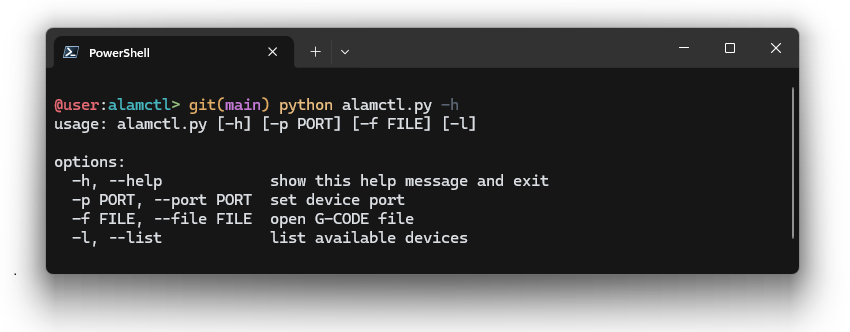
\includegraphics[width=0.95\textwidth]{cli-usage}
    \caption{Command line usage}
    \label{fig:cli-usage}
\end{figure}

Note that all parameters are optional. If no parameters are passed, as explained in the flowchart in Figure \ref{fig:system-flowchart}, the application will attempt to connect to one of the available ports. However, the recommended method is to search for available ports and then try to connect to the one whose description matches that of the controller, as shown in Figure \ref{fig:cli-connection}.

\begin{figure}[H]
    \centering
    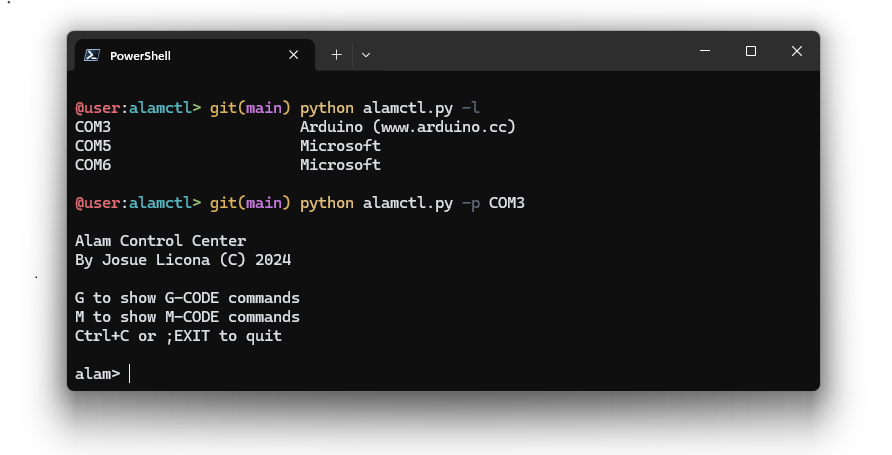
\includegraphics[width=0.95\textwidth]{cli-connection}
    \caption{Command line connection}
    \label{fig:cli-connection}
\end{figure}

When a successful connection with the robot is established, the application displays a welcome message and a short help guide to start using the robot interactively (see Figure \ref{fig:cli-manual}). However, it is also possible to pass a G-Code script as a parameter for the program to send commands automatically (Figure \ref{fig:cli-file}). This is the most efficient and powerful way to use the platform to control a robot.


\begin{figure}[H]
    \centering
    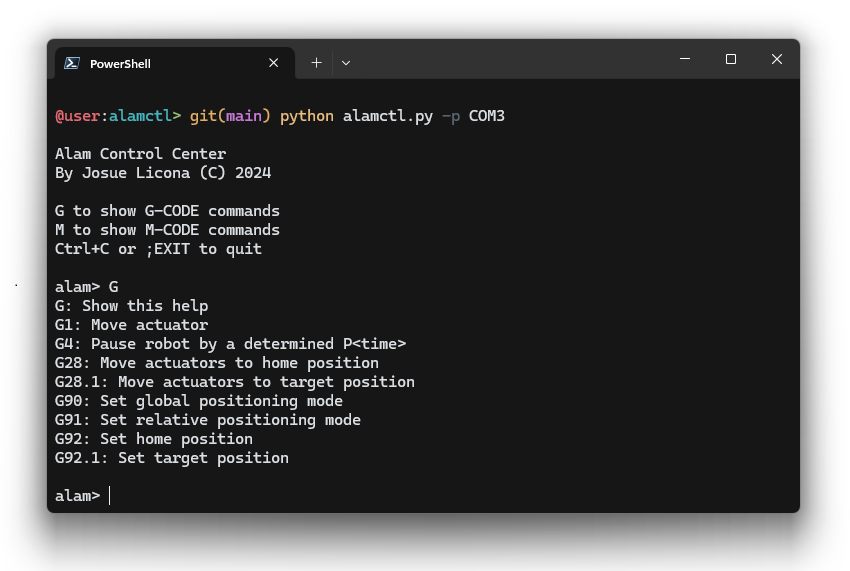
\includegraphics[width=0.95\textwidth]{cli-manual}
    \caption{Command line manual input}
    \label{fig:cli-manual}
\end{figure}

\begin{figure}[H]
    \centering
    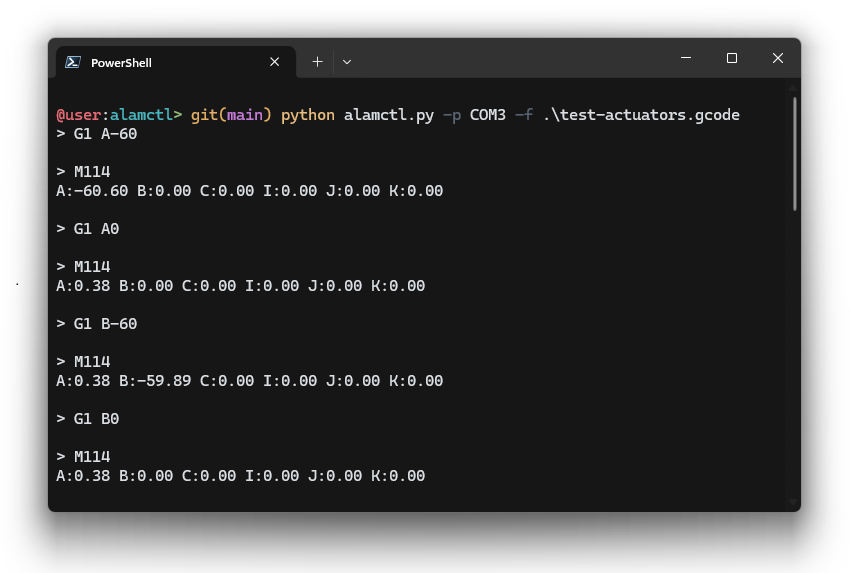
\includegraphics[width=0.95\textwidth]{cli-file}
    \caption{Command line file parsing}
    \label{fig:cli-file}
\end{figure}

\section{PID Control and Tuning}

Given that the actuators are equipped with DC motors, the controllable variable is the speed, but the position can be determined thanks to the magnetic encoder, which counts the number of motor revolutions. Based on this, a PID control is implemented to use the position as the input variable, allowing the controller to manipulate the speed to reach the desired position. To implement this control, the \textit{QuickPID}\footnote{\url{https://github.com/Dlloydev/QuickPID}} library was used, which can be integrated with the \textit{sTune} library to determine the actuator tunings automatically. An attempt was made to use this latter library to find the tunings; however, its methods are designed for systems with an S-shaped response to a constant input, which does not apply to our system. Therefore, the results from this library were often unsatisfactory. For this reason, a more powerful tool, such as MATLAB and Simulink, was used to find the tunings.

\subsection{Test Data}

\begin{figure}[h]
    \centering
    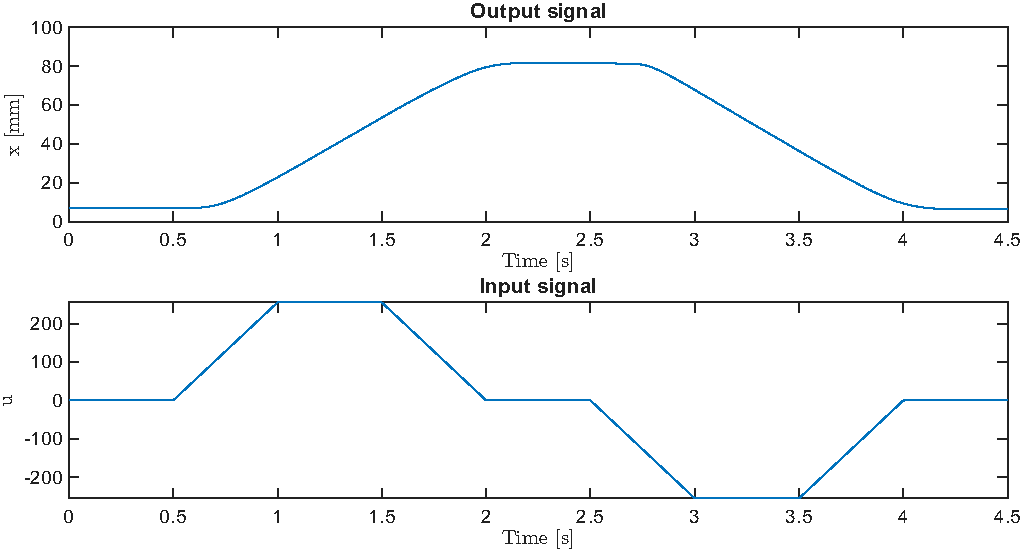
\includegraphics[page=1,width=0.95\textwidth]{input-output-signals}
    \caption{Input and output signals}
    \label{fig:io-signals}
\end{figure}

First, a test to obtain data from the actuators was conducted to understand the system. This test lasts 4.5 seconds and can be executed with the command \gcodeinline/M300/. It sends a PWM signal to the actuators that varies over time, showing the linear position of the actuator at each time instant, as seen in Figure \ref{fig:io-signals}.


\subsection{System Identification}

Based on the obtained data, the system's transfer function is identified using MATLAB's \textit{System Identification Toolbox}. The process carried out is shown in Figure \ref{fig:tf-indent-process}. The model fit to the real data is depicted in Figure \ref{fig:tf-result}. The MATLAB code used is provided in Appendix \ref{apx:pid-code}.

\begin{figure}[H]
    \centering
    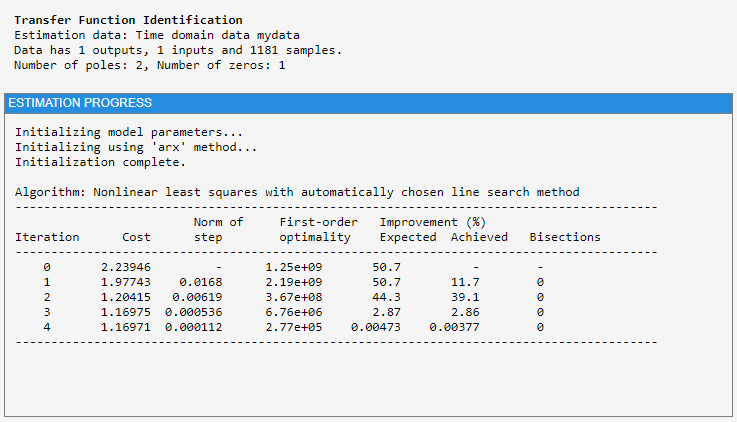
\includegraphics[width=0.7\textwidth]{tf-ident-process}
    \caption{Transfer function identification in MATLAB}
    \label{fig:tf-indent-process}
\end{figure}

\begin{figure}[H]
    \centering
    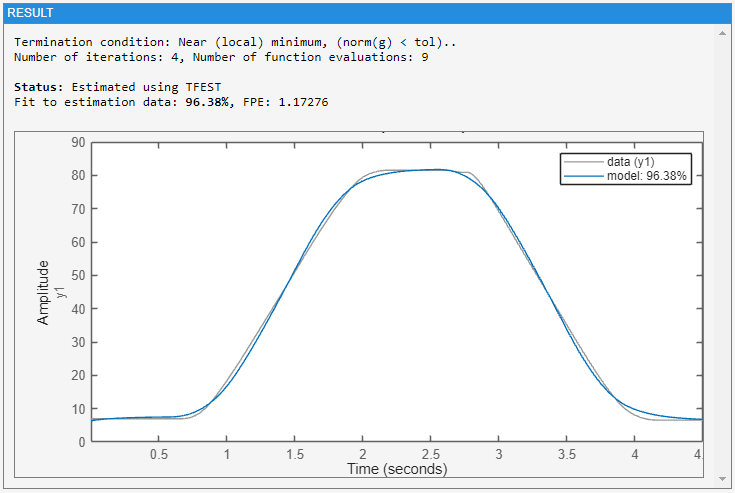
\includegraphics[width=0.7\textwidth]{tf-ident-result}
    \caption{Transfer function model in MATLAB}
    \label{fig:tf-result}
\end{figure}

The transfer equation of the linear actuator that was identified is shown in Equation \ref{eq:tf}, where the variable of the function is \( z^{-1} \).

\begin{equation}
    \label{eq:tf}
    tf=\frac{(4.808-4.596z^{-1})\times10^{-4}}{1-1.982z^{-1}+0.9824z^{-2}}
\end{equation}


\subsection{PID Tuning}

The tunings of the PID controller were determined using the \textit{pidTuner} utility from MATLAB. The type of controller that provided the best response was the PI controller, which is a PID controller with \( K_d = 0 \). In our case, this control is discrete, and the resulting constants are shown in Table \ref{tab:pid-tunings}. These variables are specified in the controller of the \textit{QuickPID} library in Arduino.

\begin{equation}
    \label{eq:pid-equation}
    C = Kp + Ki * \frac{Ts}{z-1}
\end{equation}

\begin{table}[h]
    \centering
    \caption{PID tunings}
    \label{tab:pid-tunings}
    \begin{tabular}{ll}
    \toprule
    Property & Value \\
    \midrule
    Proportional constant, $Kp$  & 21.4 \\
    Integrative constant, $Ki$ & 1.97 \\
    Sample time, $Ts$ & $0.00381$s \\
    \bottomrule
    \end{tabular}
\end{table}

\begin{figure}[H]
    \centering
    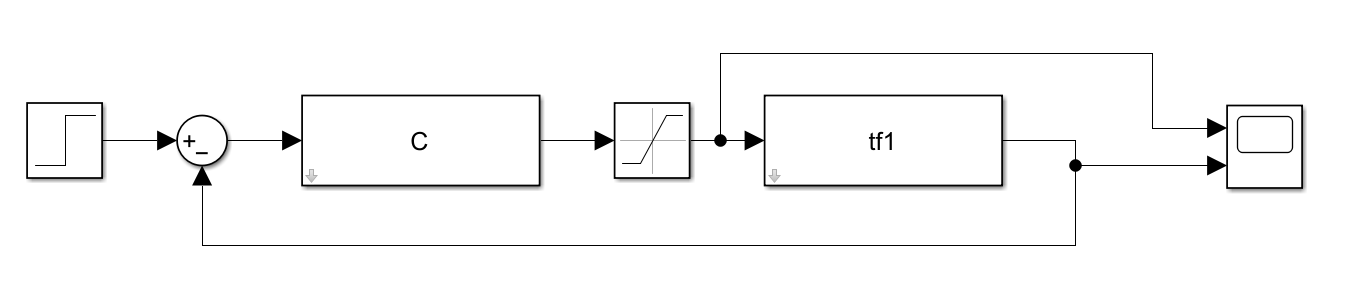
\includegraphics[width=\textwidth]{system-blocks}
    \caption{Blocks diagram of control system}
    \label{fig:system-blocks}
\end{figure}

A general block diagram of the control system is shown in Figure \ref{fig:system-blocks}, where \texttt{C} represents the transfer function of the PID controller (equation \ref{eq:pid-equation}) and \texttt{tf1} represents the transfer function of the actuator. The system's response to a 100 mm input is shown in Figure \ref{fig:system-response}. The blue curve indicates that the system responds quickly, taking just under two seconds theoretically to reach the desired value; however, it exhibits overshoot and takes nearly four seconds to settle into a steady state. Often, when the robot is in motion, it is unnecessary to wait for it to reach exact intermediate positions. Therefore, the firmware was programmed to allow new commands to be entered once the desired position is passed, sacrificing accuracy for speed.

\begin{figure}[H]
    \centering
    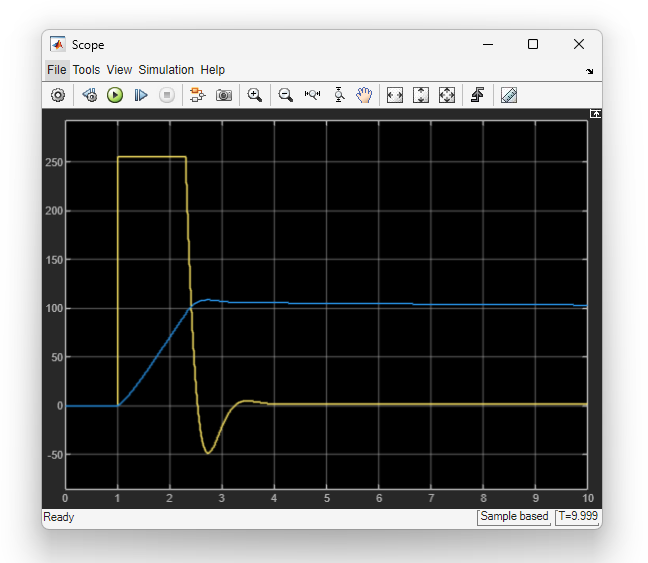
\includegraphics[width=0.6\textwidth]{system-response}
    \caption{System response of simulation in Simulink}
    \label{fig:system-response}
\end{figure}

Additionally, the control signal, shown in yellow, experiences saturation, highlighting the need to implement an anti-windup control. Fortunately, the \textit{QuickPID} library offers a function for this, making implementation straightforward.
